\documentclass [11pt,twoside]{article}
\usepackage[utf8]{inputenc}
\usepackage[T1]{fontenc}

%Page margins, header and footer positions
\usepackage{geometry}
 \geometry{
 a4paper,
 total={210mm,297mm},
 left=25mm,
 right=25mm,
 top=30mm,
 bottom=25mm,
 headsep=7mm}

\interfootnotelinepenalty=10000

%To display filling dots in the TOC for all entries
\usepackage[titles]{tocloft}
\renewcommand{\cftsecleader}{\cftdotfill{\cftdotsep}}

%Define new header and footer style
\usepackage{fancyhdr}

\pagestyle{fancy}
\fancyhf{}
\lhead{\color{Gray}{\small{Polaris project by VINCENZO MANTO \& ROBERT MEDVEDEC}}}
\lfoot{\textcolor{Gray}{\small{Copyright © 2022, VINCENZO MANTO \& ROBERT MEDVEDEC – All rights reserved}}}
\rfoot{\textcolor{Gray}{\thepage}}
\renewcommand{\headrulewidth}{0pt}

%PACKAGES
\usepackage{wasysym}
\usepackage{pifont}

\newcommand{\supported}{\ding{52}\xspace}
\newcommand{\unsupported}{\ding{55}\xspace}
\newcommand{\partsupported}{\textcolor{black!40}{\ding{52}}\xspace}
\newcommand{\lowsupported}{\textcolor{black!20}{\ding{52}}\xspace}
\newcommand{\unknowsupported}{\textbf{?}\xspace}

%Font: Times
\usepackage{times}
%Change monospaced font
\renewcommand{\ttdefault}{lmtt}

%tables
\usepackage{tabu}
\usepackage{tabularx}
\usepackage{ltablex}
\usepackage{longtable}
\usepackage{float} % To allow the use of H modifier in long tables

%landscape mode
\usepackage{pdflscape}
\usepackage{rotating}
\usepackage{caption}

%make landscape mode be sensitive to even and odd pages
%start
\def\myrotate{\ifodd\c@page\else-\fi 90}
\makeatletter
\global\let\orig@begin@landscape=\landscape%
\global\let\orig@end@landscape=\endlandscape%
\gdef\@true{1}
\gdef\@false{0}
\gdef\landscape{%
    \global\let\within@landscape=\@true%
    \orig@begin@landscape%
}%
\gdef\endlandscape{%
    \orig@end@landscape%
    \global\let\within@landscape=\@false%
}%
\@ifpackageloaded{pdflscape}{%
    \gdef\pdf@landscape@rotate{\PLS@Rotate}%
}{
    \gdef\pdf@landscape@rotate#1{}%
}
\let\latex@outputpage\@outputpage
\def\@outputpage{
    \ifx\within@landscape\@true%
        \if@twoside%
            \ifodd\c@page%
                \gdef\LS@rot{\setbox\@outputbox\vbox{%
                    \pdf@landscape@rotate{-90}%
                    \hbox{\rotatebox{90}{\hbox{\rotatebox{180}{\box\@outputbox}}}}}%
                }%
            \else%
                \gdef\LS@rot{\setbox\@outputbox\vbox{%
                    \pdf@landscape@rotate{+90}%
                    \hbox{\rotatebox{90}{\hbox{\rotatebox{0}{\box\@outputbox}}}}}%
                }%
            \fi%
        \else%
            \gdef\LS@rot{\setbox\@outputbox\vbox{%
                \pdf@landscape@rotate{+90}%
                \hbox{\rotatebox{90}{\hbox{\rotatebox{0}{\box\@outputbox}}}}}%
            }%
        \fi%
    \fi%
    \latex@outputpage%
}
\makeatother
%end

%graphics
\usepackage{graphicx}
\usepackage[dvipsnames, table]{xcolor}
%If you upload images from PC, you need to insert code for the path here (different for Windows and Unix OS)

%References
%\usepackage{xpatch}
%\usepackage[backend=biber, style=numeric, citestyle=numeric, sorting=none]{biblatex}
%\addbibresource{main.bib}

%Other
\usepackage{ifthen}
\usepackage{xspace}
\usepackage{enumitem}
\usepackage{amssymb}
\usepackage[pdftex, colorlinks]{hyperref}
\newcommand{\comment}[1]{{\color{Red}$\blacktriangleright$ Comment: #1 $\blacktriangleleft$}}


% Some utilities\ldots
\usepackage{soul}
\usepackage{tikz}

\usetikzlibrary{calc}
\usetikzlibrary{decorations.pathmorphing}


\makeatletter

\newcommand{\defhighlighter}[3][]{%
  \tikzset{every highlighter/.style={color=#2, fill opacity=#3, #1}}%
}

\defhighlighter{yellow}{.5}

\newcommand{\highlight@DoHighlight}{
  \fill [ decoration = {random steps, amplitude=1pt, segment length=15pt}
        , outer sep = -15pt, inner sep = 0pt, decorate
       , every highlighter, this highlighter ]
        ($(begin highlight)+(0,8pt)$) rectangle ($(end highlight)+(0,-3pt)$) ;
}

\newcommand{\highlight@BeginHighlight}{
  \coordinate (begin highlight) at (0,0) ;
}

\newcommand{\highlight@EndHighlight}{
  \coordinate (end highlight) at (0,0) ;
}

\newdimen\highlight@previous
\newdimen\highlight@current

\DeclareRobustCommand*\highlight[1][]{%
  \tikzset{this highlighter/.style={#1}}%
  \SOUL@setup
  %
  \def\SOUL@preamble{%
    \begin{tikzpicture}[overlay, remember picture]
      \highlight@BeginHighlight
      \highlight@EndHighlight
    \end{tikzpicture}%
  }%
  %
  \def\SOUL@postamble{%
    \begin{tikzpicture}[overlay, remember picture]
      \highlight@EndHighlight
      \highlight@DoHighlight
    \end{tikzpicture}%
  }%
  %
  \def\SOUL@everyhyphen{%
    \discretionary{%
      \SOUL@setkern\SOUL@hyphkern
      \SOUL@sethyphenchar
      \tikz[overlay, remember picture] \highlight@EndHighlight ;%
    }{%
    }{%
      \SOUL@setkern\SOUL@charkern
    }%
  }%
  %
  \def\SOUL@everyexhyphen##1{%
    \SOUL@setkern\SOUL@hyphkern
    \hbox{##1}%
    \discretionary{%
      \tikz[overlay, remember picture] \highlight@EndHighlight ;%
    }{%
    }{%
      \SOUL@setkern\SOUL@charkern
    }%
  }%
  %
  \def\SOUL@everysyllable{%
    \begin{tikzpicture}[overlay, remember picture]
      \path let \p0 = (begin highlight), \p1 = (0,0) in \pgfextra
        \global\highlight@previous=\y0
        \global\highlight@current =\y1
      \endpgfextra (0,0) ;
      \ifdim\highlight@current < \highlight@previous
        \highlight@DoHighlight
        \highlight@BeginHighlight
      \fi
    \end{tikzpicture}%
    \the\SOUL@syllable
    \tikz[overlay, remember picture] \highlight@EndHighlight ;%
  }%
  \SOUL@
}

\makeatother

% Common abbrev. are set as commands to ensure proper spacing after the dot
\RequirePackage{xspace}
\newcommand{\ie}{i.e.\@\xspace}
\newcommand{\aka}{a.k.a.\@\xspace}
\newcommand{\Ie}{I.e.\@\xspace}
\newcommand{\cf}{cf.\@\xspace}
\newcommand{\Cf}{Cf.\@\xspace}
\newcommand{\eg}{e.g.\@\xspace}
\newcommand{\Eg}{E.g.\@\xspace}
\newcommand{\etal}{et al.\@\xspace}
\newcommand{\etc}{etc.\@\xspace}
\newcommand{\wrt}{w.r.t.\@\xspace}
\newcommand{\Wrt}{W.r.t.\@\xspace}



\date{}


\begin{document}

%TITLE PAGE

\begin{titlepage}


%LOGO

{\begin{table}[t!]
\centering
\begin{tabu} to \textwidth { X[1.3,r,p] X[1.7,l,p] }
\textcolor{Blue}
{\textbf{\small{Travlendar+ project YOUR NAMES}}} & 
\includegraphics[scale=0.5]{Images/PolimiLogo}
\end{tabu}
\end{table}}~\\ [7cm]

%TITLE 

\begin{flushleft}

%Replace the text string with your title
{\textcolor{Blue}{\textbf{\Huge{Requirement Analysis and Specification
        Document}}}} \\ [1cm]

\end{flushleft}

\end{titlepage}

%Define deliverable specific info
%Replace cell contents where needed
\begin{table}[h!]
\begin{tabu} to \textwidth { X[0.3,r,p] X[0.7,l,p] }
\hline

\textbf{Deliverable:} & RASD\\
\textbf{Title:} & Requirement Analysis and Verification Document \\
\textbf{Authors:} & YOUR NAMES \\
\textbf{Version:} & 1.0 \\ 
\textbf{Date:} & 31-January-2016 \\
\textbf{Download page:} & LINK TO YOUR REPOSITORY \\
\textbf{Copyright:} & Copyright © 2017, YOUR NAMES – All rights reserved \\
\hline
\end{tabu}
\end{table}




\setcounter{page}{2}


%------------------------------------------------------------------------------------------------------------------------------------------------
\newpage
\addcontentsline{toc}{section}{Table of Contents}
\tableofcontents
\newpage
\addcontentsline{toc}{section}{List of Figures}
\listoffigures
\addcontentsline{toc}{section}{List of Tables}
\listoftables

%------------------------------------------------------------------------------------------------------------------------------------------------
\clearpage
{\color{Blue}{\section{Introduction}}}
\label{sect:introduction}
\subsection{Purpose}
\hspace{\parindent}This document provides a detailed description, mainly of the  architecture and the UI, of the 'Polaris' mobile application.\\
'Polaris' application is a system used to enhance travelling experience through idea sharing among people, exploration of other users' travels, documentation and easy manipulation of trip destinations and ideas. The system itself is made so the user has every single information regarding his travel in one place, without having to remember or worry about any details.\\
'Polaris' is mainly a mobile application, with a possibility of being also expanded as a web application in the future.  
\newpage

\subsection{Scope}
\hspace{\parindent}'Polaris' is an application that helps all travellers around the world to easily and efficiently manage their travels and thus enhance their travelling experience. The target audience for this application is everyone who uses a smartphone and has at least some experience in using mobile applications, as some of the patterns and application usages might not be intended for the novices in the field. Thus the target audience ranges from 15 to 50 years old, although there are no strict boundaries.\linebreak


The application is mainly intended to be used when a user is planning and making their own trip and has a liberty to organize their free time and places to visit.\linebreak


Another important usage of the application is sharing trip ideas with friends and other users around the world. Planning trips by itself is a daunting and time consuming task, and with the lack of adequate applications on the market, we wanted to create something that is going to allow users to easily share and modify their previous trips and therefore improve the overall travelling experience for others. 
\break
The most important functions of the application are arranging a trip, finding points of interest in the area, organizing visits to those points, exploring accommodation and restaurants in the area, and crafting your own views of the travel by providing additional comments on the whole experience.


\newpage

\subsection{Definitions, Acronyms, Abbreviations}
\subsubsection{Definitions}
\begin{itemize} 
	\item \textbf{Application}: a computer (mobile) program that is designed for a particular purpose. 
	\item \textbf{Smartphone}: a mobile phone that performs many of the functions of a computer, typically having a touchscreen interface, internet access, and an operating system capable of running downloaded apps. 
	\item \textbf{Google Maps}: a web mapping service developed by Google, used both as a standalone app and as an integrated mapping solution in most of the apps.
	\item \textbf{iOS}: operating system developed by Apple, used by their portable devices like iPads and iPhones.
	\item \textbf{Android}: most popular operating system for smartphones and tablets, developed by Google and partners.
	\item \textbf{Backend}: the part of a computer system or application that is not directly accessed by the user, typically responsible for storing and manipulating data.
\end{itemize}
\subsubsection{Acronyms}
\begin{itemize}
	\item \textbf{API}: Application programming interface, computing interface which defines interactions between multiple software intermediaries 
	\item \textbf{UI}: User interface	
	\item \textbf{GUI}: Graphical user interface
	\item \textbf{DB}: Database
	\item \textbf{REST}: Representational state transfer - software architectural style used in web services
\end{itemize}
\subsubsection{Abbreviations}
\begin{itemize}
	\item \textbf{App}: Application.
\end{itemize}

\newpage
\subsection{Revision History}
\begin{itemize}
	\item \textbf{Version 0.1}: First .tex document created and added all together; 28th December 2021
\end{itemize}

\newpage
\subsection{Reference Documents}
\begin{itemize}
	\item nothing
\end{itemize}



%------------------------------------------------------------------------------------------------------------------------------------------------
\clearpage
{\color{Blue}{\section{Overall Description}}}
\label{sect:overview}
Here you can see how to include an image in your document.

\begin{sidewaysfigure}
\centering
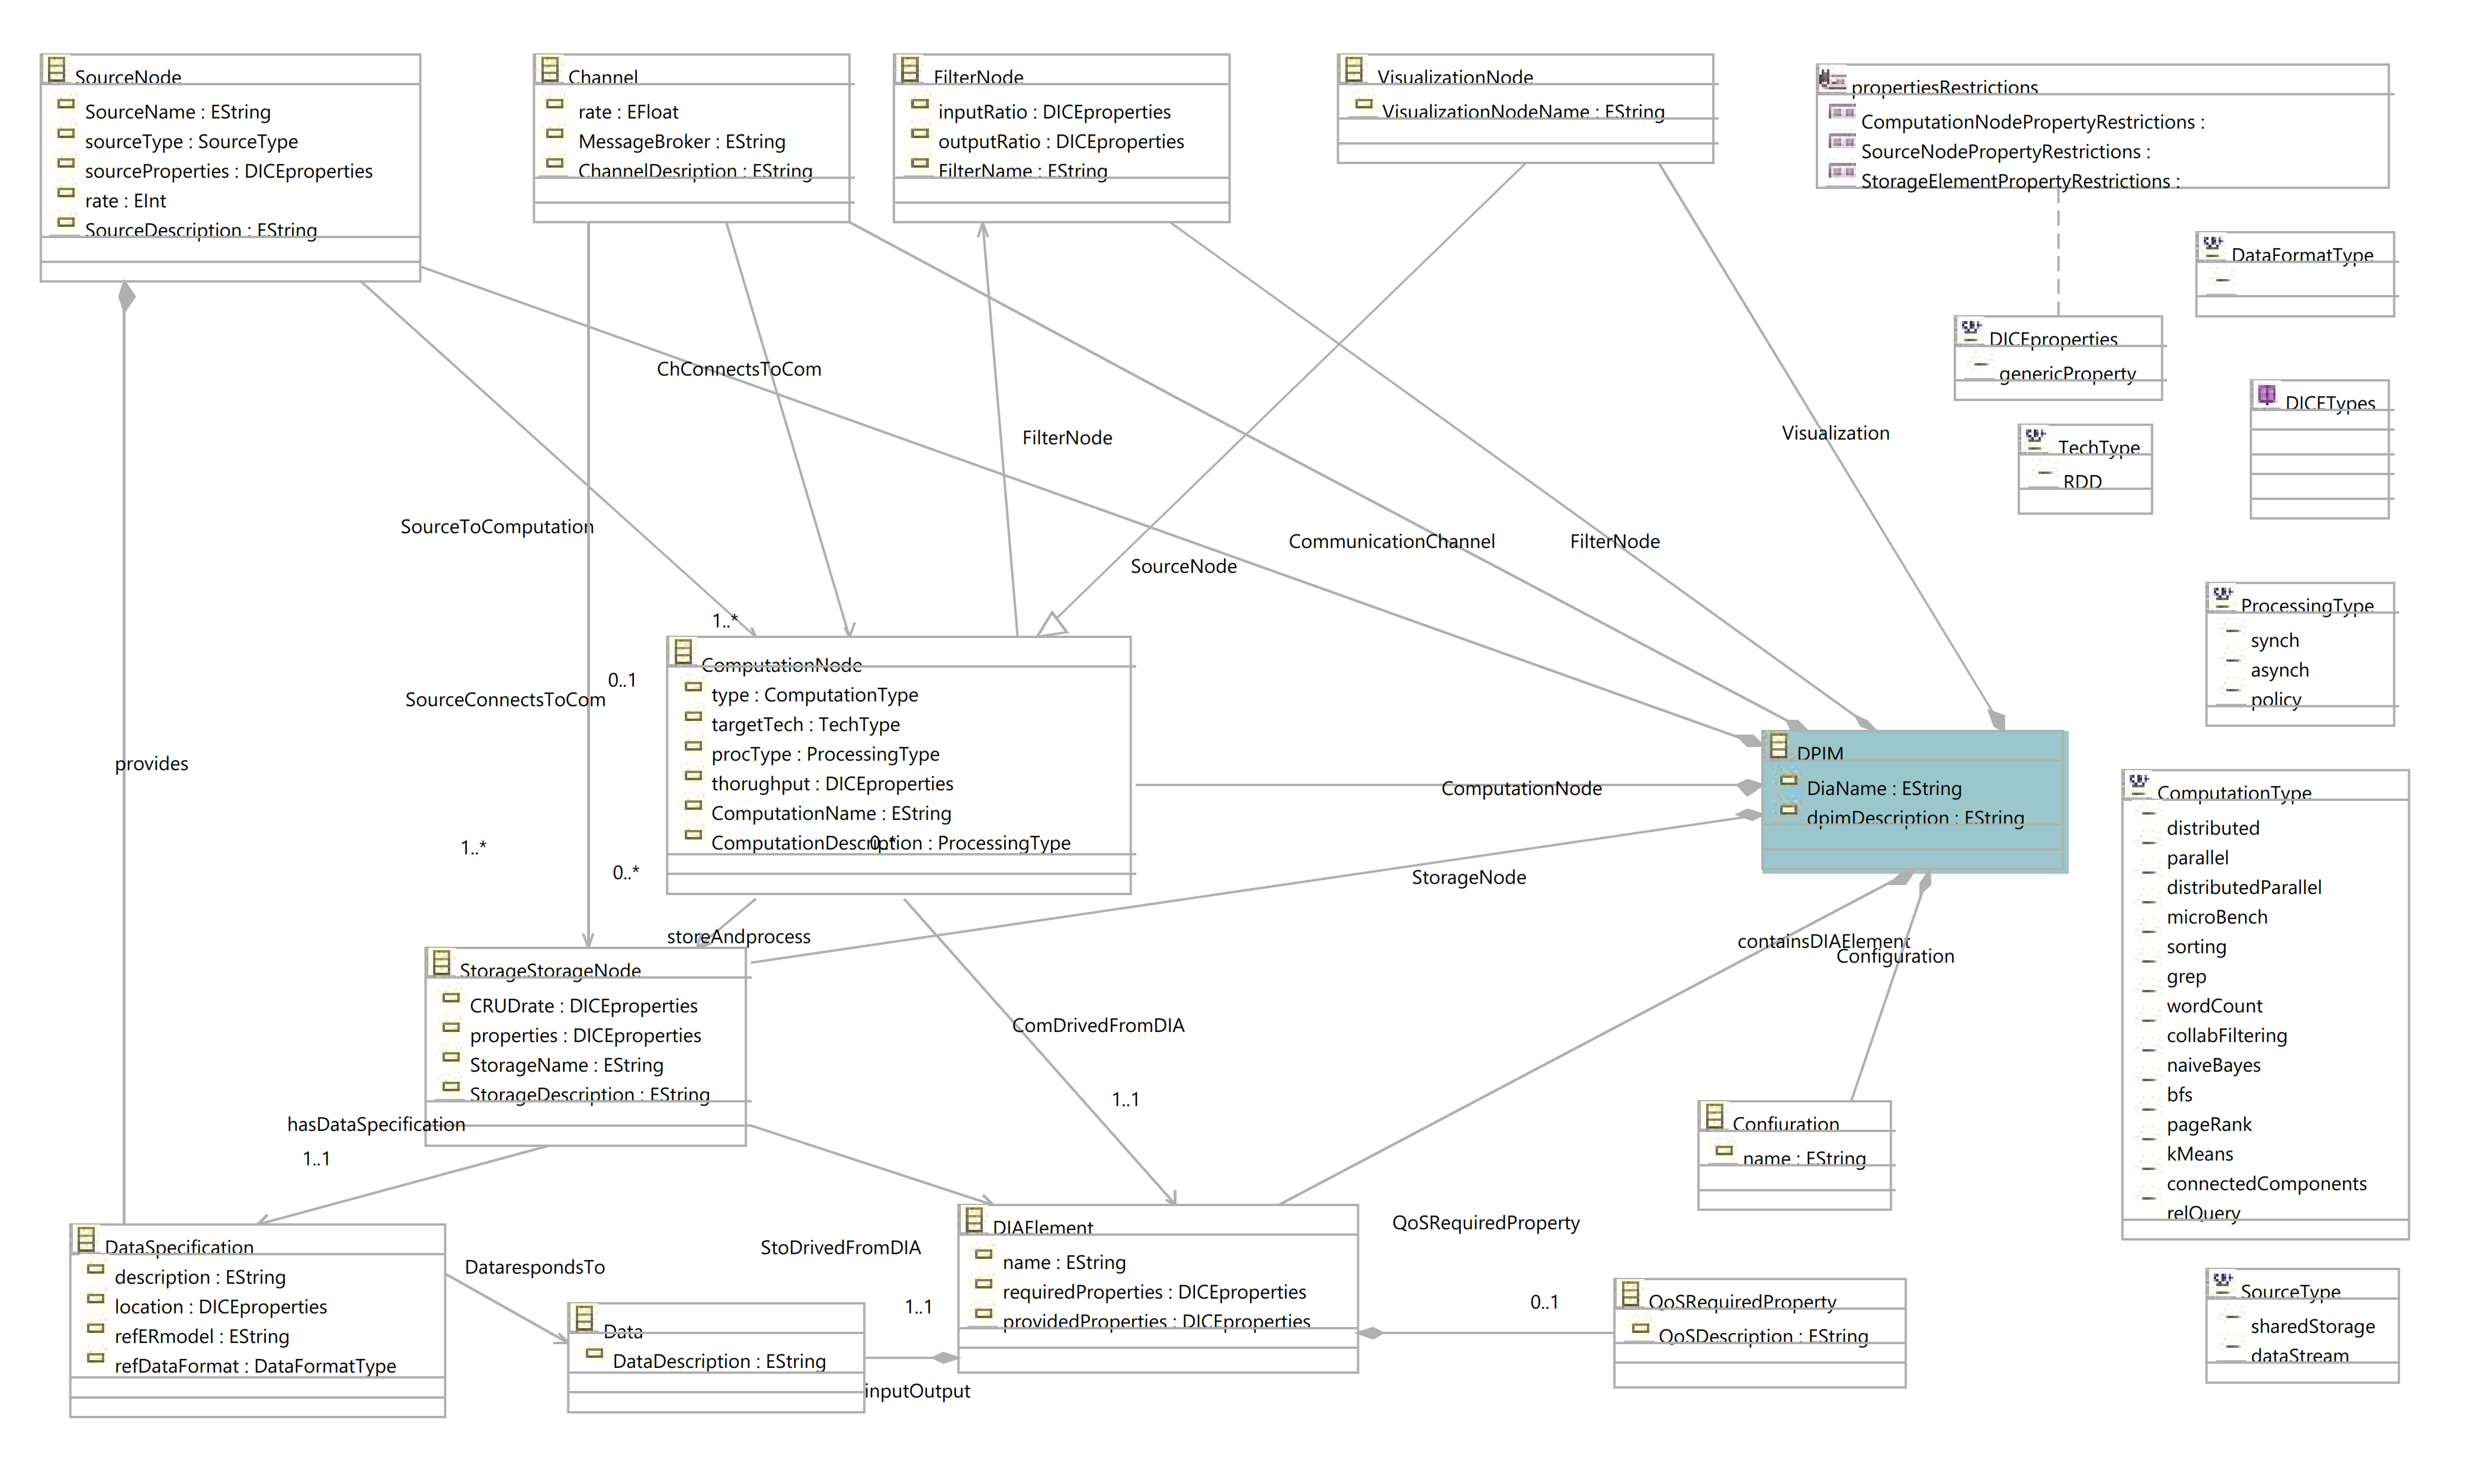
\includegraphics[width=\textwidth]{Images/11.png}
\caption{\label{fig:metamodel}DICE DPIM metamodel.}
\end{sidewaysfigure}

\begin{figure}
\centering
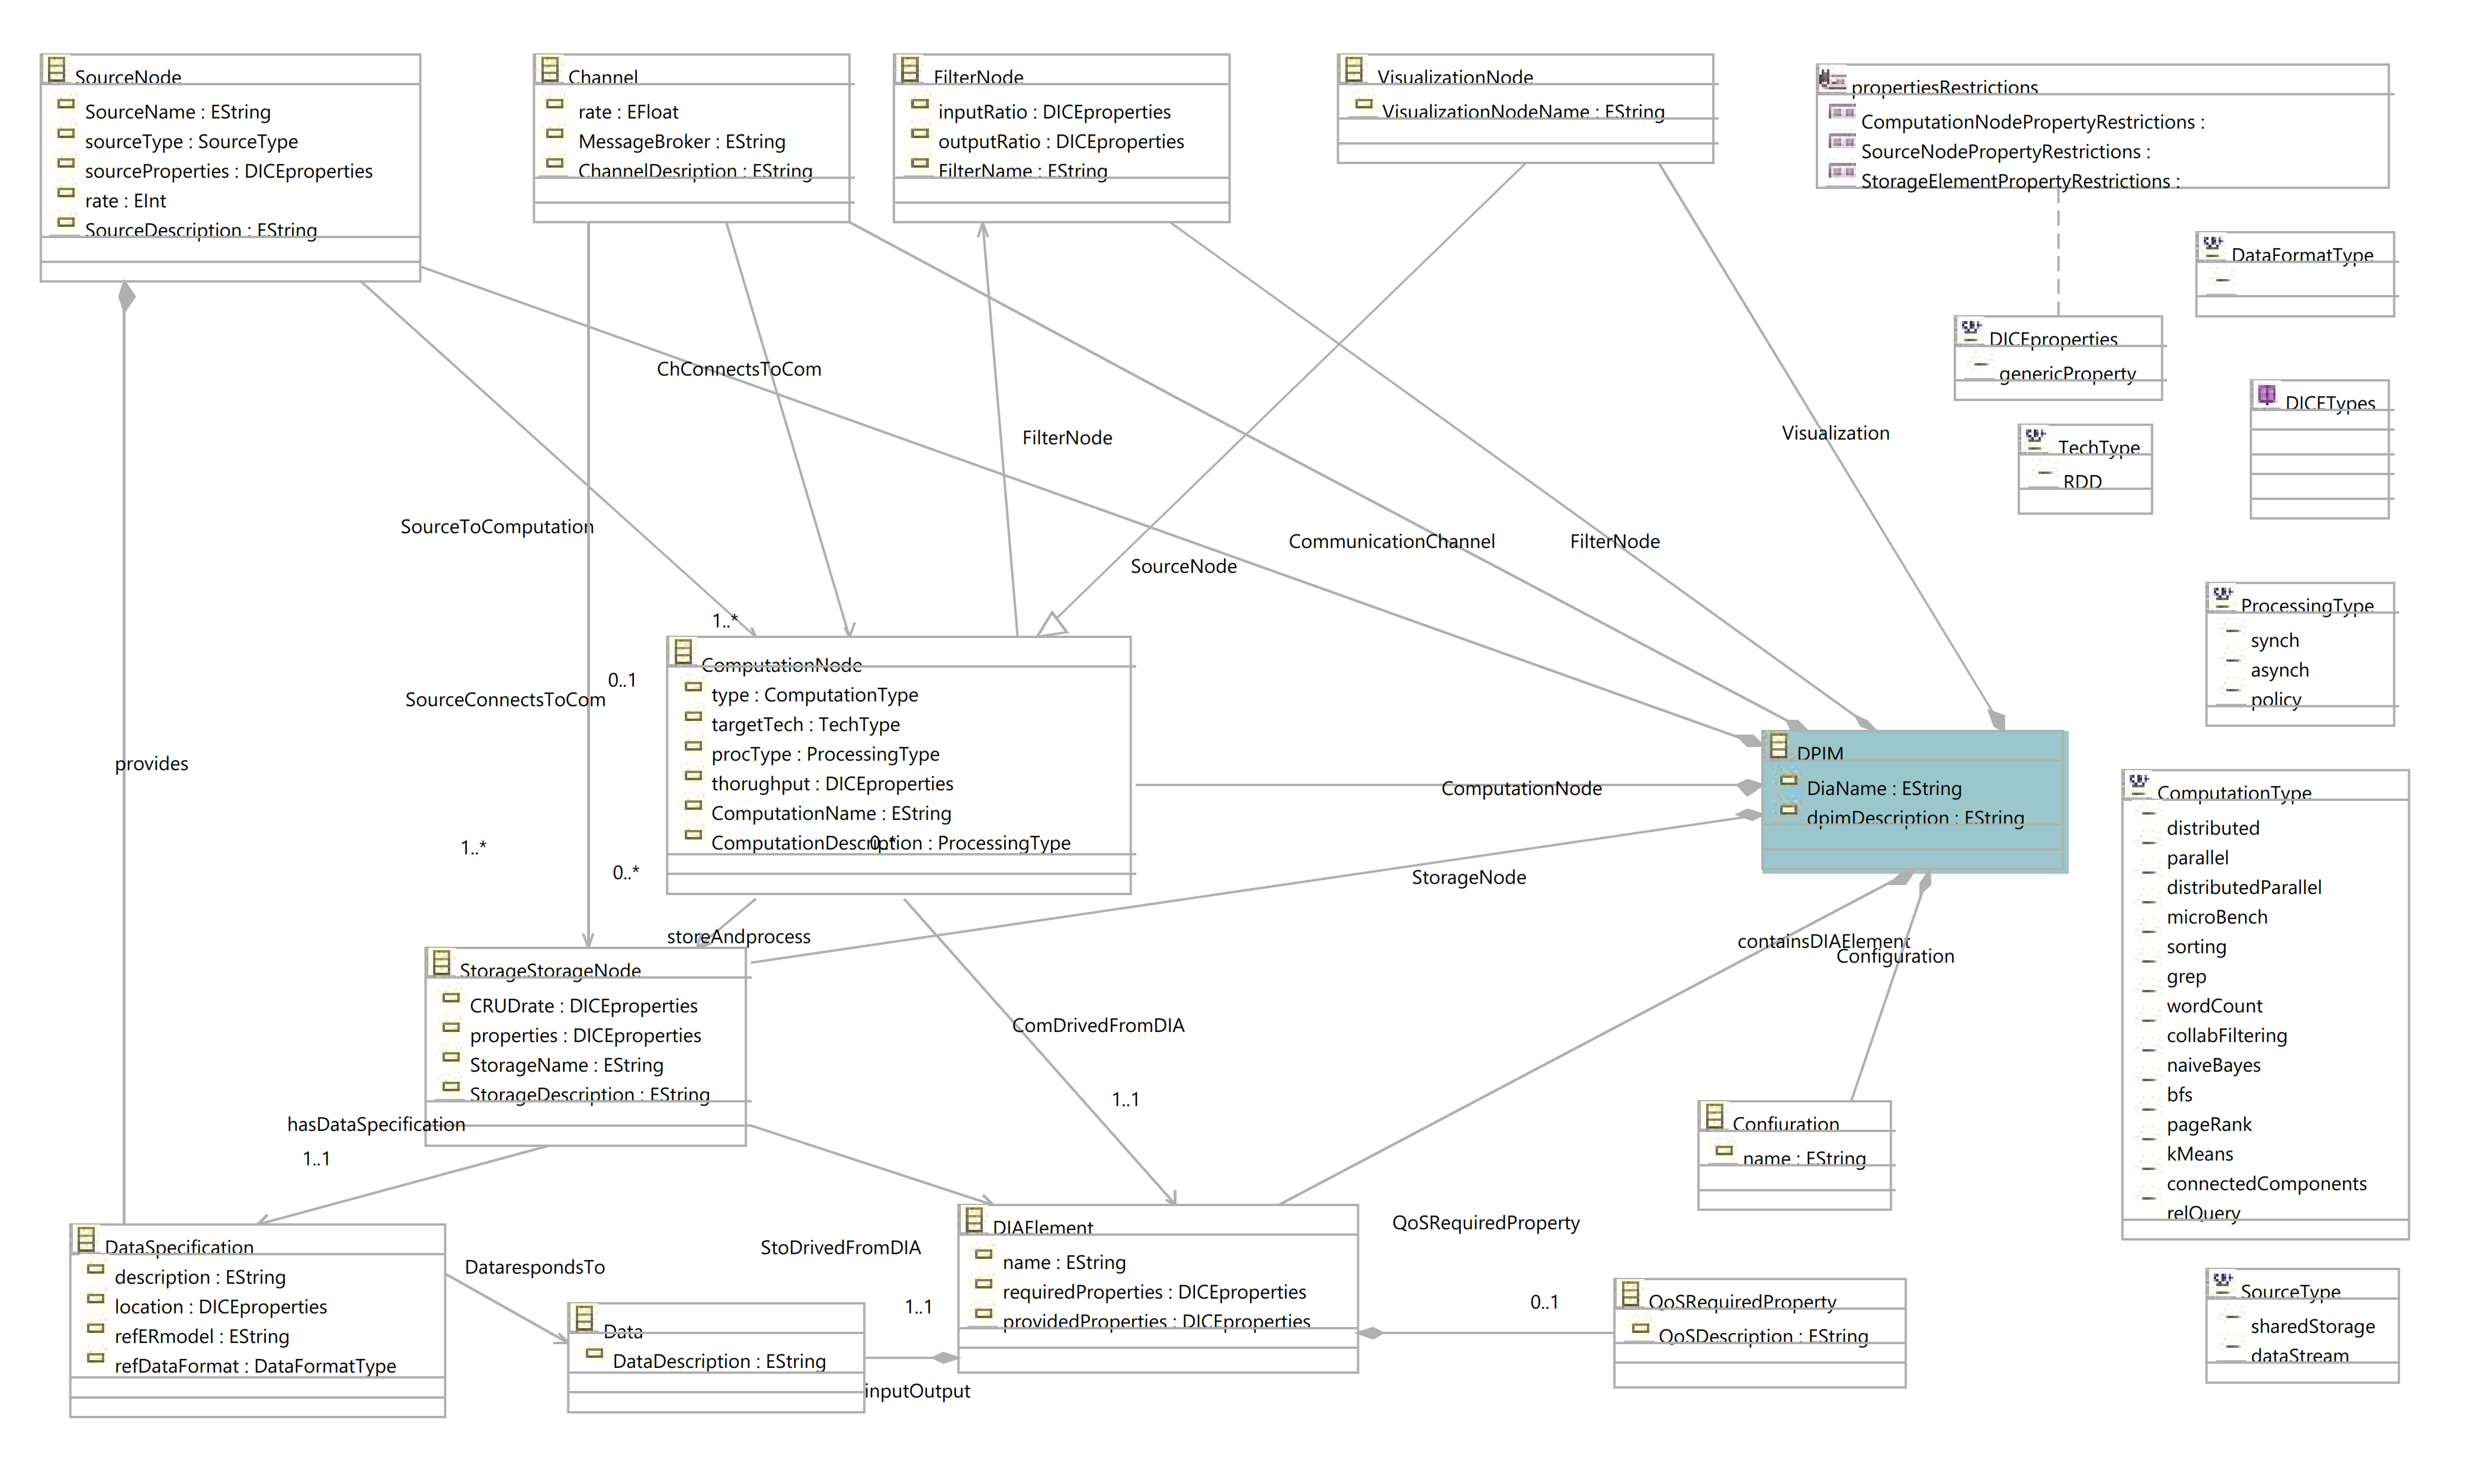
\includegraphics[width=\textwidth]{Images/11.png}
\caption{\label{fig:metamodel2}DICE DPIM metamodel in portrait form.}
\end{figure}

Here is the command to refer to another element (section, figure, table, ...) in the document: \emph{As discussed in Section~\ref{sect:overview} and as shown in Figure~\ref{fig:metamodel}, ...}. Here is how to introduce a bibliographic citation~\cite{DAM}. Bibliographic references should be included in a \texttt{.bib} file. 

Table generation is a bit complicated in Latex. You will soon become proficient, but to start you can rely on tools or external services. See for instance this \href{https://www.tablesgenerator.com}{https://www.tablesgenerator.com}. 


%------------------------------------------------------------------------------------------------------------------------------------------------
\clearpage
{\color{Blue}{\section{Specific Requirements}}}
\label{sect:requirements}
\subsection{External Interface Requirements}
\subsubsection{User Interfaces}
\hspace{\parindent}The CLup application interface will have to serve two types of users: customers and store managers. Opening screen of the application allows the user to pick a store or to login as a store manager. Depending on the choice, another screen is presented. For a customer, a screen with the options to retrieve a ticket, book a visit or change the store. For a store manager, a screen containing their camera view, and buttons to confirm the scanned ticket, notify the system about a customer exit and to log out of the application. 
\subsubsection{Hardware Interfaces}
\hspace{\parindent}Depending on the current user the CLup application will require access to some hardware interfaces. If the current user is a customer, the application will require the device's camera and if the current user is the store manager the GPS location data will be needed. The application will require no further hardware interfaces.
\subsubsection{Software Interfaces}
\hspace{\parindent}The CLup application will not require any specific software interfaces.
\subsubsection{Communication Interfaces}
\hspace{\parindent}The most important communication will occur between the device and the database. The decision on the specific communication interface which will be used depends on the database, and is, therefore, left to the developers.

\newpage
\subsection{Functional Requirements}
\begin{enumerate}
	\item [\textbf{G1}] Allow a User to "line up"/retrieve a number.
	\begin{enumerate}
		\item [\textbf{G1.1}] Allow a User to retrieve a number through the application.
		\begin{enumerate}
			\item [\textbf{R1}] The user must be able to select a specific store in which they want to do the shopping.
			\item [\textbf{R2}] The user must be able to request a number and a ticket.
			\item [\textbf{R3}] The user must be able to receive a number and a ticket.
		\end{enumerate}
		\item [\textbf{G1.2}] Allow a User to retrieve a number physically from the printer.
		\begin{enumerate}
			\item [\textbf{R4}] The user must be able to physically retrieve a ticket from the printer containing a number and a QR code.		
		\end{enumerate}
		\item [\textbf{D8}] The user has internet connection for the device at all times.
	\end{enumerate}
	\item [\textbf{G2}] Allow a Store Manager to control the entrance of a User via QR code scanning.
	\begin{enumerate}
		\item [\textbf{R5}] The store manager must be able to scan a QR code.
		\item [\textbf{R6}] The store manager must be informed by the application if a user tries to enter the store out of order.
		\item [\textbf{R7}] The store manager must be informed when the capacity of the store is full.
		\item [\textbf{R8}] The store manager must be able to alert the system whenever a customer exits the store.
		\item [\textbf{D6}] The system can correctly save data about enter and exit times of anonymous customers, in order to calculate estimated wait time.
		\item [\textbf{D8}] The user has internet connection for the device at all times.
	\end{enumerate}
	\item [\textbf{G3}] Allow a User to get precise calculations of the wait time.
	\begin{enumerate}
		\item [\textbf{R9}] Allow the user to receive a precise estimation of wait time when retrieving a number.
		\item [\textbf{R10}] The system must provide the user with an estimation of wait time based on data.
		\item [\textbf{D4}] The system can use data about the registered user to calculate estimated wait time.
		\item [\textbf{D6}] The system can correctly save data about enter and exit times of anonymous customers, in order to calculate estimated wait time.
		\item [\textbf{D8}] The user has internet connection for the device at all times.
	\end{enumerate}
	\item [\textbf{G4}] Allow a User to get updates/notifications on the estimated wait time.
	\begin{enumerate}
		\item [\textbf{R11}] The system must be able to update its estimated wait time in real time.
		\item [\textbf{R12}] The system must be able to send an update to the user in specific intervals regarding estimated wait time until it's their turn.
		\item [\textbf{D4}] The system can use data about the registered user to calculate estimated wait time.
		\item [\textbf{D6}] The system can correctly save data about enter and exit times of anonymous customers, in order to calculate estimated wait time.
		\item [\textbf{D8}] The user has internet connection for the device at all times.
	\end{enumerate}
	\item [\textbf{G5}] Allow a User to "book a visit" to the store.
	\begin{enumerate}
		\item [\textbf{G5.1}] Allow a User to "book a visit" to the store without indicating the expected duration of the visit.
		\begin{enumerate}
			\item [\textbf{R13}] The user must be able to request to see all the available timeslots in that specific store.
			\item [\textbf{R14}] The system must be able to provide the user with the list of all available timeslots upon the request.
			\item [\textbf{R15}] The user must be able to select a specific timeslot.
			\item [\textbf{R16}] The user must be able to receive a confirmation of his timeslot reservation, along with a number and a ticket.
			\item [\textbf{R17}] Allow the user to be at most five minutes late for his reservation before canceling his ticket.
		\end{enumerate}
		\item [\textbf{G5.2}] Allow a User to "book a visit" to the store with indicating the expected duration of the visit.
		\begin{enumerate}
			\item [\textbf{R18}] The user must be able to specify expected duration of his visit to the store.
		\end{enumerate}
 		\item [\textbf{D3}] The user's device provides accurate GPS information.
		\item [\textbf{D7}] The system can correctly save data to and pull data from available time slot schema in the database. 
		\item [\textbf{D8}] The user has internet connection for the device at all times.
	\end{enumerate}
	\item [\textbf{G6}] Allow a Store Manager to login to his store manager account with credentials.
	\begin{enumerate}
		\item [\textbf{R19}] The store manager must be provided with the login credentials upon request to the system administrator.
		\item [\textbf{D1}] The store manager's username must be unique. 
		\item [\textbf{D2}] The store manager's password must be secure. 
	\end{enumerate}
\end{enumerate}

\newpage
\begin{table}[]
\centering
\begin{tabular}{|
>{\columncolor[HTML]{EFEFEF}}l |l|l|}
\hline
\cellcolor[HTML]{C0C0C0}\textbf{Requirement, {[}Rn{]}} & \cellcolor[HTML]{C0C0C0}\textbf{Goals, {[}Gn{]}} & \cellcolor[HTML]{C0C0C0}\textbf{Domains, {[}Dn{]}} \\ \hline
R1  & G1.1 & D8         \\ \hline
R2  & G1.1 & D8         \\ \hline
R3  & G1.1 & D8         \\ \hline
R4  & G1.2 & D8         \\ \hline
R5  & G2   & D6, D8     \\ \hline
R6  & G2   & D6, D8     \\ \hline
R7  & G2   & D6, D8     \\ \hline
R8  & G2   & D6, D8     \\ \hline
R9  & G3   & D4, D6, D8 \\ \hline
R10 & G3   & D4, D6, D8 \\ \hline
R11 & G4   & D4, D6, D8 \\ \hline
R12 & G4   & D4, D6, D8 \\ \hline
R13 & G5.1 & D3, D7, D8 \\ \hline
R14 & G5.1 & D3, D7, D8 \\ \hline
R15 & G5.1 & D3, D7, D8 \\ \hline
R16 & G5.1 & D3, D7, D8 \\ \hline
R17 & G5.1 & D3, D7, D8 \\ \hline
R18 & G5.2 & D3, D7, D8 \\ \hline
R19 & G6   & D1, D2     \\ \hline
\end{tabular}
\caption{Mapping table}
\label{tab:my-table}
\end{table}
\subsection{Performance Requirements}



%------------------------------------------------------------------------------------------------------------------------------------------------
\clearpage
{\color{Blue}{\section{Formal Analysis Using Alloy}}}
\label{sect:alloy}
Organize this section according to the rules defined in the project description. 


%------------------------------------------------------------------------------------------------------------------------------------------------
\clearpage
{\color{Blue}{\section{Effort Spent}}}
\label{sect:effort}
Provide here information about how much effort each group member spent in working at this document. We would appreciate details here.



%------------------------------------------------------------------------------------------------------------------------------------------------
\clearpage
\addcontentsline{toc}{section}{References}
\bibliographystyle{plain}
\bibliography{main}
%------------------------------------------------------------------------------------------------------------------------------------------------




\end{document}
